% =====================================================================
%  Poly Citra CoolBrick — A4 report
%  Version 2: CoolBrick kennels for dogs. Structured to the competition entry
%  requirements (Summary ... Bibliography) with a cost price analysis.
%
%  Compile:  pdflatex poly_citra_coolbrick_a4.tex   (run twice)
%  Red [ ... ] marks a placeholder the team must fill in or verify.
% =====================================================================
\documentclass[11pt,a4paper]{article}

\usepackage[a4paper,margin=2cm,top=2.2cm,bottom=2.2cm]{geometry}
\usepackage[T1]{fontenc}
\usepackage{lmodern}
\usepackage[scaled=0.95]{helvet}
\renewcommand{\familydefault}{\sfdefault}
\usepackage{microtype}
\usepackage{graphicx}
\usepackage{booktabs}
\usepackage{tabularx}
\usepackage{array}
\usepackage{amsmath}
\usepackage{siunitx}
\usepackage{enumitem}
\usepackage{caption}
\usepackage{subcaption}
\usepackage{float}
\usepackage{xcolor}
\usepackage{tikz}
\usetikzlibrary{arrows.meta,positioning,calc,decorations.pathmorphing,patterns}
\usepackage{pgfplots}
\pgfplotsset{compat=1.18}
\usepackage[most]{tcolorbox}
\usepackage{titlesec}
\usepackage{fancyhdr}
\usepackage{needspace}
\usepackage[hidelinks]{hyperref}
\providecommand{\rupee}{Rs\,}

\graphicspath{{img/}}

% ---------- palette (from the original deck) ----------
\definecolor{citrus}{HTML}{E8731A}
\definecolor{leaf}{HTML}{2E7D32}
\definecolor{sky}{HTML}{1E88C8}
\definecolor{plum}{HTML}{8E2A8E}
\definecolor{ink}{HTML}{1F2A36}
\definecolor{heat}{HTML}{C62828}

\color{ink}
\setlength{\parindent}{0pt}
\setlength{\parskip}{6pt}
\setlist{itemsep=2pt,topsep=2pt}

\captionsetup{font=small,labelfont={bf,color=citrus},labelsep=period}

% ---------- headings ----------
\titleformat{\section}{\Large\bfseries\color{ink}}
  {\colorbox{citrus}{\color{white}\,\thesection\,}}{0.6em}{}[\vspace{-4pt}{\color{citrus}\titlerule[1.2pt]}]
\titleformat{\subsection}{\large\bfseries\color{leaf}}{\thesubsection}{0.6em}{}
\titlespacing*{\section}{0pt}{14pt}{8pt}
\let\origsection\section
\renewcommand{\section}{\clearpage\origsection}
\titleformat{\part}[block]{\Huge\bfseries\color{leaf}}{}{0pt}{}
\renewcommand{\contentsname}{\color{ink}Contents}
\titlespacing*{\subsection}{0pt}{10pt}{4pt}

% ---------- page frame: thin border + header/footer ----------
\pagestyle{fancy}
\fancyhf{}
\renewcommand{\headrulewidth}{0pt}
\fancyhead[L]{\small\color{citrus}\textbf{Poly Citra} \color{ink}CoolBrick}
\fancyhead[R]{\small\color{gray}Project Rebrick}
\fancyfoot[C]{\small\color{gray}\thepage}
\usepackage{eso-pic}
\AddToShipoutPictureBG{%
  \begin{tikzpicture}[remember picture,overlay]
    \draw[citrus,line width=1.2pt,rounded corners=6pt]
      ($(current page.north west)+(1.0cm,-1.0cm)$) rectangle ($(current page.south east)+(-1.0cm,1.0cm)$);
    \draw[leaf!60,line width=0.4pt,rounded corners=5pt]
      ($(current page.north west)+(1.15cm,-1.15cm)$) rectangle ($(current page.south east)+(-1.15cm,1.15cm)$);
  \end{tikzpicture}}

% ---------- helpers ----------
\newcommand{\todo}[1]{\textcolor{heat}{\textbf{[#1]}}}
\newcommand{\new}{\tikz[baseline=-0.6ex]\node[fill=citrus,text=white,font=\tiny\bfseries,rounded corners=2pt,inner sep=2pt]{NEW};}
\newtcolorbox{card}[2][]{enhanced,colback=#2!6,colframe=#2,boxrule=0pt,
  leftrule=3pt,arc=2pt,left=6pt,right=6pt,top=4pt,bottom=4pt,fontupper=\small,
  before skip=6pt,after skip=6pt,#1}
\newtcolorbox{keybox}[1]{enhanced,colback=#1!8,colframe=#1,boxrule=0.8pt,arc=3pt,
  left=8pt,right=8pt,top=6pt,bottom=6pt,before skip=8pt,after skip=8pt}


\begin{document}

% =====================================================================
%  COVER
% =====================================================================
\begin{titlepage}
\thispagestyle{empty}
\vspace*{0.4cm}
{\fontsize{34}{40}\selectfont\bfseries \textcolor{leaf}{Poly} \textcolor{citrus}{Citra} \textcolor{leaf}{Bricks}\par}
\vspace{4pt}
{\Large\itshape Transforming Waste into Sustainable Building Materials\par}
\vspace{6pt}
{\color{citrus}\rule{0.45\textwidth}{2pt}}\par
\vspace{2pt}
{\large Innovative Eco-Friendly Construction Solutions\par}
\vspace{4pt}
{\large\color{sky}\bfseries Version 2: \textcolor{citrus}{CoolBrick} kennels that protect dogs from India's heat\par}

\vspace{1cm}
\begin{center}
\begin{minipage}{0.49\textwidth}
  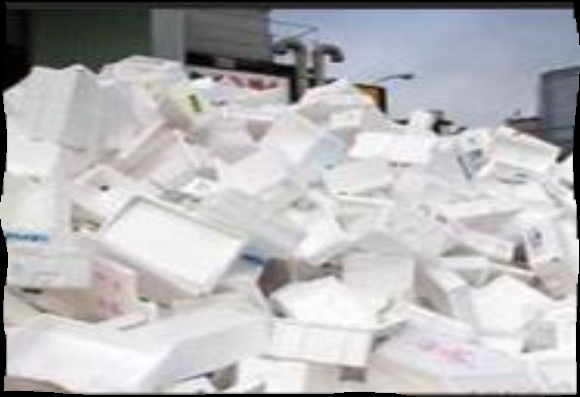
\includegraphics[width=\linewidth,height=4.2cm,keepaspectratio=false]{styrofoam.jpg}
\end{minipage}\hfill
\begin{minipage}{0.49\textwidth}
  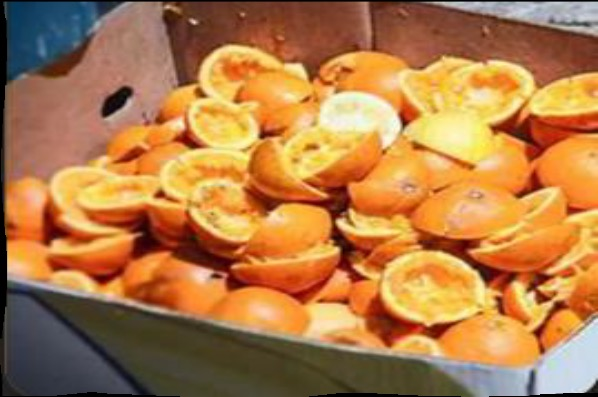
\includegraphics[width=\linewidth,height=4.2cm,keepaspectratio=false]{peels.jpg}
\end{minipage}\\[6pt]
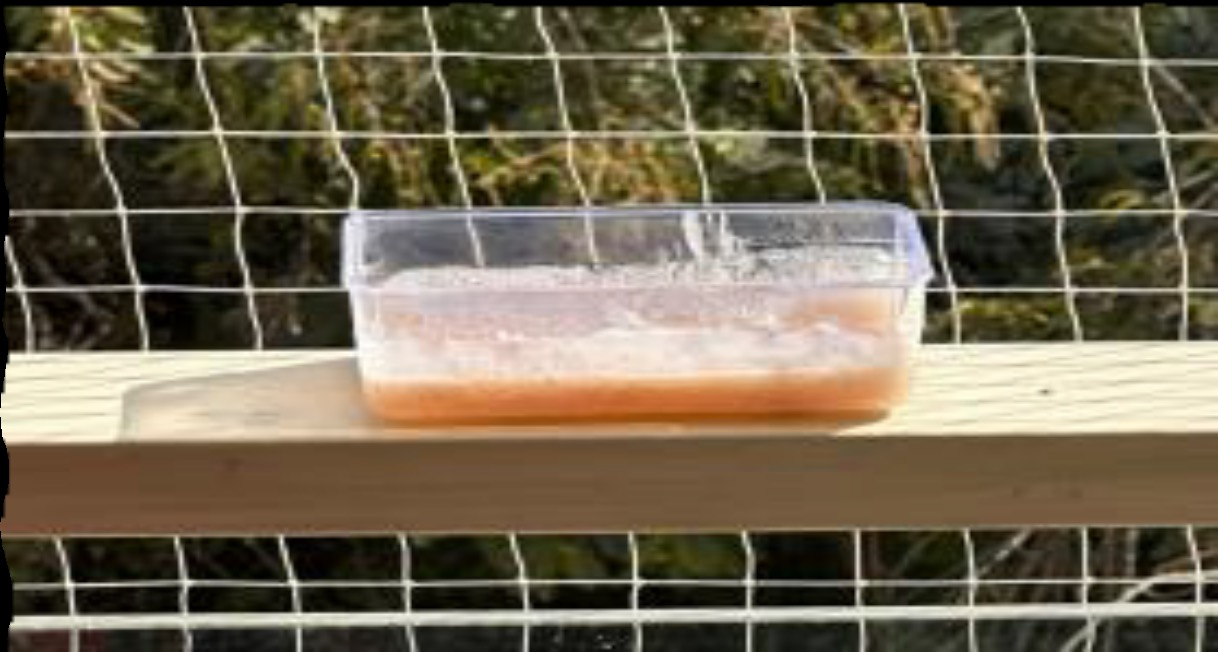
\includegraphics[width=\textwidth,height=7.6cm,keepaspectratio=false]{prototype.jpg}
\end{center}

\vfill
\begin{tabular}{@{}ll}
\textbf{Project:} & Project Rebrick \\
\textbf{Team:} & Rian Sikka and Daiwik Abroo \\
\textbf{Grade:} & Grade 9 (IGCSE) \\
\textbf{School:} & Scottish High International School \\
\end{tabular}
\end{titlepage}

% =====================================================================
\setcounter{tocdepth}{1}
\tableofcontents


% =====================================================================
\section{Summary}

Every year India throws away large amounts of \textbf{Styrofoam} (expanded
polystyrene, EPS) packaging and \textbf{orange peel}. Both usually end up in
landfill or are burned. Our project, \textbf{Poly Citra Bricks}, turns these
two wastes into building bricks. We extract \textbf{D-limonene}, a natural
solvent, from orange peel by steam distillation. Limonene dissolves Styrofoam
into a thick polystyrene gel, which we mould and cure into a light,
waterproof brick. This first version has already been built, tested and
recognised at national-level competitions \todo{list awards}.

In this edition we use the brick to protect \textbf{dogs from heat}. India
has crores of street dogs and many more pet, shelter and working dogs. Dogs
cannot sweat like us; they cool down mainly by panting, which works less well
as the air gets hotter. Kennels made of plastic, tin or plain brick heat up in
the sun and can become hotter than the air outside. The \textbf{CoolBrick}
adds five passive-cooling features: hollow air cells, pockets of a
coconut-oil phase-change material (PCM), a white calcium-carbonate
``cool-face'' coating, a filler of biochar made from the leftover peel, and
perforated \emph{jaali} vent blocks. No electricity is needed.

We wrote a computer heat-flow simulation of a dog kennel
(\SI{1.0}{m} $\times$ \SI{0.8}{m} $\times$ \SI{0.8}{m}) with a resting dog
inside on a hot day (air 27--\SI{41}{\celsius}). We also worked out what the
bricks and the kennel cost to make.

\begin{keybox}{citrus}
\centering
\begin{tabular}{ccc}
{\LARGE\bfseries\color{citrus} 40.0\,°C} & {\LARGE\bfseries\color{leaf} 4.7\,°C cooler} & {\LARGE\bfseries\color{sky} \rupee3/day}\\[2pt]
\small hottest it feels inside the & \small walls next to the dog, & \small cost of a CoolBrick kennel\\
\small CoolBrick kennel (clay 43.8\,°C, & \small compared with a clay & \small over a 10-year life\\
\small plastic 45.3\,°C, outdoor air 41\,°C) & \small kennel at peak & \small (\rupee11,059 per kennel)
\end{tabular}
\end{keybox}

These are model predictions using assumed material values and price
estimates. Our next step is to build model kennels and test them with a
heated ``dog dummy'' (Section~4). No animals are used in our experiments.


% =====================================================================
\section{Significance and Uniqueness of the Project}

\subsection{The problem: two wastes}
\begin{minipage}[t]{0.52\textwidth}
\vspace{0pt}
\begin{itemize}
  \item \textbf{Styrofoam waste} contributes to landfill overflow and
        environmental pollution.
  \item \textbf{Orange peel waste} ends up in landfills or is incinerated,
        leading to environmental pollution.
  \item Without effective recycling methods, these wastes worsen pollution
        and waste-management issues.
  \item A sustainable solution is needed to repurpose them into
        eco-friendly alternatives.
\end{itemize}
\end{minipage}\hfill
\begin{minipage}[t]{0.45\textwidth}
\vspace{0pt}
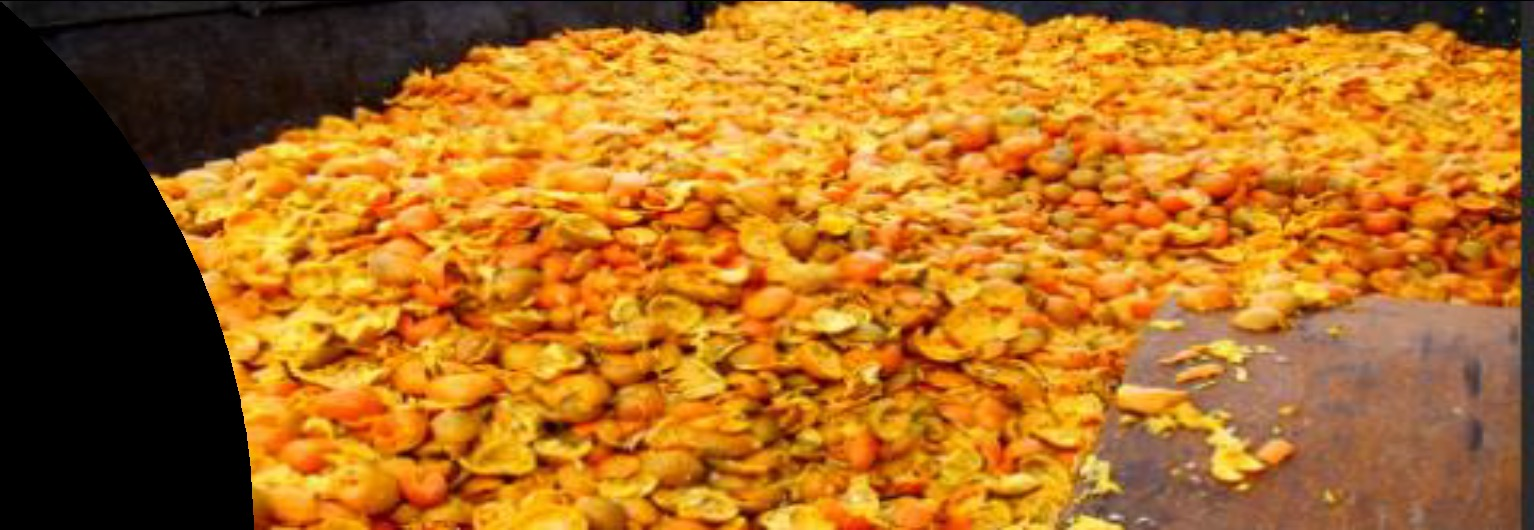
\includegraphics[width=\linewidth,height=3.3cm,keepaspectratio=false]{peel-waste.jpg}\\[-2pt]
{\footnotesize\color{gray}Orange-peel waste}\\[4pt]
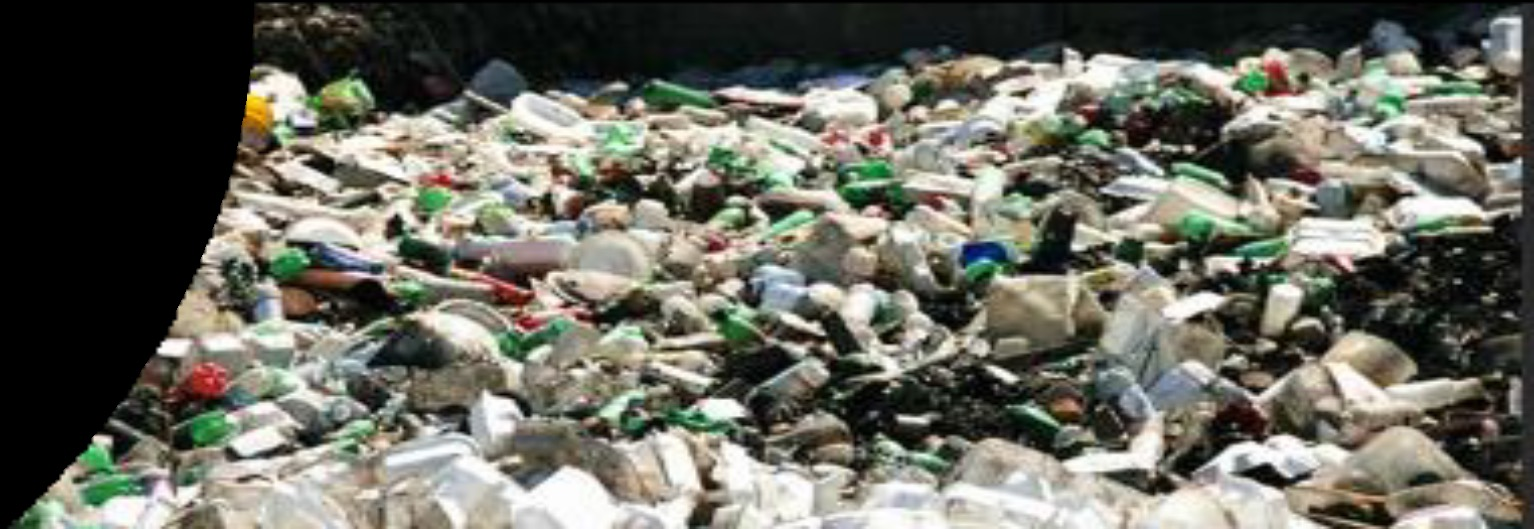
\includegraphics[width=\linewidth,height=3.3cm,keepaspectratio=false]{plastic-waste.jpg}\\[-2pt]
{\footnotesize\color{gray}Plastic and Styrofoam waste in landfill}
\end{minipage}

\subsection{The problem: dogs in India's heat}
\begin{itemize}
  \item India's 2019 Livestock Census counted about \textbf{1.5 crore street
        dogs}; other surveys estimate as many as \textbf{6 crore}. Millions
        more are pets, guard dogs, shelter dogs and working dogs.
  \item Dogs \textbf{cannot sweat} through their skin; they sweat a little
        through their paw pads and lose heat mainly by \textbf{panting}.
        Panting works less well as the air gets hotter and more humid.
  \item A dog's normal body temperature is about \SI{38.5}{\celsius}. Above
        about \SI{40}{\celsius} it is heat-stressed, and about
        \SI{41}{\celsius} or more is heatstroke, which can kill.
  \item Indian summers bring long heatwaves above \SI{40}{\celsius}. Many
        shelters and street-dog feeders use plastic, tin or plain-brick
        kennels. In the sun, these heat up and radiate heat onto the dog.
  \item Animal shelters and street-dog projects usually cannot pay for fans,
        coolers or air-conditioning, or the electricity to run them.
\end{itemize}

\begin{card}{citrus}
\textbf{The insight:} a dog in a kennel feels the heat of the walls and roof
as well as the air. If the kennel stays cool, the dog can rest safely through
the hottest hours, with no electricity.
\end{card}

\subsection{What makes this project unique}
\begin{itemize}
  \item \textbf{Two wastes, one product.} Styrofoam and orange peel both
        become part of the brick. No clay is mined and no kiln is fired.
  \item \textbf{The whole orange is used.} The peel gives the solvent
        (limonene), and what is left after distillation becomes the biochar
        filler. The limonene is recovered and reused.
  \item \textbf{Five cooling methods in one brick.} Most kennels use none.
        The CoolBrick combines reflection, sky radiation, trapped air, heat
        storage and ventilation.
  \item \textbf{Built for dogs, with no running cost.} No electricity, no
        moving parts, easy to clean, and cheap to keep over many years.
  \item \textbf{A costed plan.} We worked out the cost price of each brick and
        each kennel, and compared it with plastic and clay kennels
        (Section~7).
\end{itemize}

\subsection{Benefits and the UN Sustainable Development Goals}
\begin{minipage}[t]{0.49\textwidth}
\begin{card}{citrus}\textbf{Minimises} landfill waste and microplastic contamination.\end{card}
\begin{card}{sky}\textbf{Reduces reliance} on natural resources like clay.\end{card}
\end{minipage}\hfill
\begin{minipage}[t]{0.49\textwidth}
\begin{card}{leaf}\textbf{Protects animals} from heat with no electricity.\end{card}
\begin{card}{plum}\textbf{Promotes} circular-economy principles.\end{card}
\end{minipage}

\begin{center}
\small
\begin{tabularx}{\textwidth}{@{}>{\bfseries}l X@{}}
\toprule
\textcolor{citrus}{SDG 11} & Sustainable Cities and Communities --- safer, kinder cities for the people and animals who share them. \\
\textcolor{citrus}{SDG 12} & Responsible Consumption and Production --- reducing waste and repurposing materials. \\
\textcolor{citrus}{SDG 13} & Climate Action --- adapting to heatwaves without using more electricity; no kiln emissions. \\
\bottomrule
\end{tabularx}
\end{center}


% =====================================================================
\section{Concept: The Science Behind the CoolBrick}

\subsection{Dissolving polystyrene with D-limonene}
Polystyrene and D-limonene are both \textbf{non-polar} hydrocarbons. Following
the rule ``like dissolves like'', limonene molecules slip between the long
polystyrene chains and separate them, so the solid foam turns into a sticky
gel. One kilogram of limonene can dissolve about 3--4 kg of Styrofoam, and
because the foam is about 98\% air its volume shrinks enormously. D-limonene
makes up over 90\% of orange-peel oil and is extracted by \textbf{steam
distillation}: steam carries the oil out of the peel, and the oil separates
from the water when it condenses. Fresh peel gives roughly 0.6--1\% oil by
mass. When the gel dries, the limonene evaporates and the polystyrene
hardens again into a solid brick. The limonene vapour can be condensed and
reused.

\begin{figure}[H]
\centering
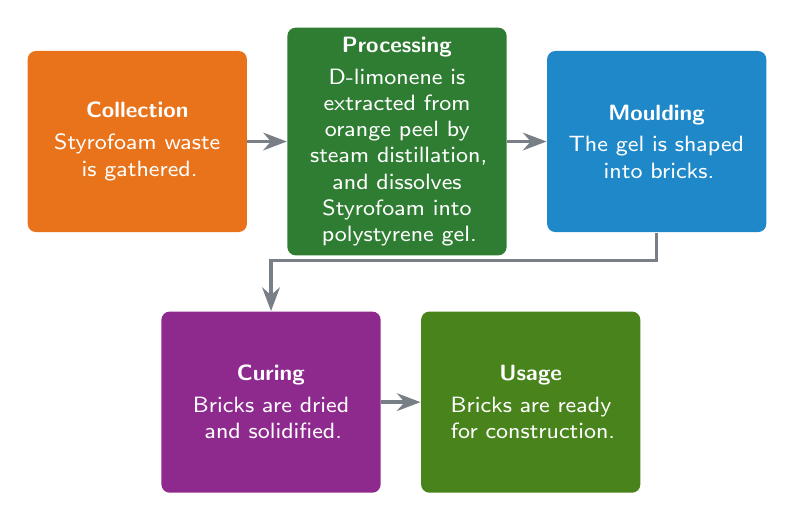
\begin{tikzpicture}[
  stp/.style={rectangle,rounded corners=3pt,minimum width=2.75cm,minimum height=2.3cm,
              text width=2.55cm,align=center,font=\footnotesize,text=white},
  arr/.style={-{Stealth[length=3mm]},line width=1.2pt,color=ink!60}]
\node[stp,fill=citrus] (a) {\textbf{Collection}\\[2pt]Styrofoam waste is gathered.};
\node[stp,fill=leaf,right=0.5cm of a] (b) {\textbf{Processing}\\[2pt]D-limonene is extracted from orange peel by steam distillation, and dissolves Styrofoam into polystyrene gel.};
\node[stp,fill=sky,right=0.5cm of b] (c) {\textbf{Moulding}\\[2pt]The gel is shaped into bricks.};
\node[stp,fill=plum,below=0.7cm of b,xshift=-1.6cm] (d) {\textbf{Curing}\\[2pt]Bricks are dried and solidified.};
\node[stp,fill=leaf!70!lime!80!black,right=0.5cm of d] (e) {\textbf{Usage}\\[2pt]Bricks are ready for construction.};
\draw[arr] (a)--(b); \draw[arr] (b)--(c);
\draw[arr] (c.south) |- ++(0,-0.35) -| (d.north);
\draw[arr] (d)--(e);
\end{tikzpicture}
\caption{The Poly Citra Brick process.}
\end{figure}

\begin{card}{leaf}
\textbf{Why it works.} Styrofoam is about 98\% air, so dissolving it shrinks
its volume dramatically and a large amount of waste fits into one brick.
D-limonene is a natural, bio-based solvent (Sony piloted the same idea for
recycling packaging foam), and no kiln firing is needed.
\end{card}

\subsection{How a dog loses heat}
A resting dog makes about \SIrange{40}{60}{W} of body heat. It must lose that
heat to its surroundings in three ways: \textbf{panting} (evaporating water
from the tongue and airways), \textbf{contact} with cooler surfaces (lying on a
cool floor or against a cool wall), and \textbf{radiation} to cooler surfaces
around it. A hot roof or wall does the opposite: it radiates heat
\emph{onto} the dog. So the temperature a dog ``feels'' in a kennel is roughly
the average of the air temperature and the temperature of the surfaces
around it. The cooler the walls and roof, the easier it is for the dog to stay
safe.

\subsection{How heat gets into a kennel}
\begin{minipage}[c]{0.46\textwidth}
\centering
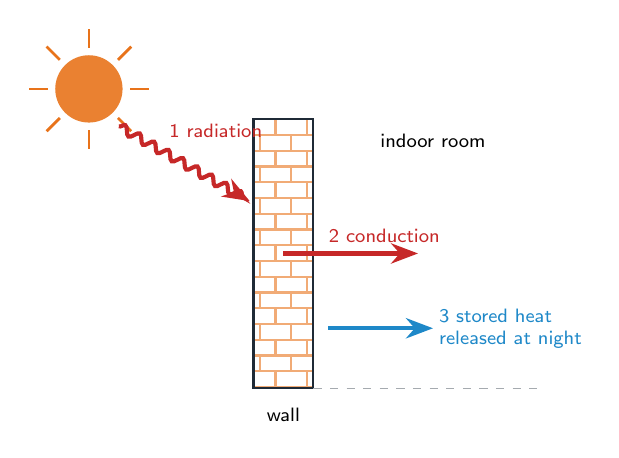
\begin{tikzpicture}[scale=0.95]
  \fill[citrus!90] (0,4.0) circle (0.45);
  \foreach \a in {0,45,...,315}{\draw[citrus,line width=1pt] ($(0,4.0)+(\a:0.55)$)--($(0,4.0)+(\a:0.8)$);}
  \fill[pattern=bricks,pattern color=citrus!60] (2.2,0) rectangle (3.0,3.6);
  \draw[ink,line width=0.8pt] (2.2,0) rectangle (3.0,3.6);
  \node[font=\scriptsize] at (2.6,-0.35) {wall};
  \node[font=\scriptsize] at (4.6,3.3) {indoor room};
  \draw[ink!40,dashed] (3.0,0) -- (6.0,0);
  \draw[-{Stealth},heat,line width=1.5pt,decorate,decoration={snake,amplitude=1.5pt,segment length=6pt}] (0.4,3.5)--(2.15,2.5)
     node[pos=0.3,above right,font=\scriptsize,text=heat]{1 radiation};
  \draw[-{Stealth},heat,line width=1.5pt] (2.6,1.8)--(4.4,1.8)
     node[pos=0.75,above,font=\scriptsize,text=heat]{2 conduction};
  \draw[-{Stealth},sky,line width=1.5pt] (3.2,0.8)--(4.6,0.8)
     node[pos=0.95,right,font=\scriptsize,text=sky,align=left]{3 stored heat\\released at night};
\end{tikzpicture}
\captionof{figure}{Three ways heat reaches the inside of a kennel.}
\end{minipage}\hfill
\begin{minipage}[c]{0.5\textwidth}
Steady heat flow through a wall:
\[
  Q = U\,A\,\Delta T,
  \qquad
  U = \frac{1}{R_{si} + \sum_i d_i/k_i + R_{so}}
\]
{\small where $U$ is the heat transmittance (\si{W/m^2K}), $d$ the layer
thickness (m), $k$ the thermal conductivity (\si{W/mK}), and
$R_{si}=0.13$, $R_{so}=0.04$~\si{m^2K/W} are the surface resistances.}

A CoolBrick must beat all three paths: reflect sunlight and radiate heat to
the sky; have a low $k$; and buffer peaks with stored ``coolth''.
\end{minipage}

\subsection{Key insight: put the air back}
\begin{minipage}[c]{0.52\textwidth}
Styrofoam insulates because it is about \textbf{98\% trapped air}
($k \approx \SI{0.035}{W/mK}$). When limonene dissolves it, the air escapes.
Solid polystyrene has $k \approx 0.10$--\SI{0.17}{W/mK}: still far better
than fired clay ($\approx\SI{0.8}{W/mK}$), but 3--5 times worse than the
foam.

\textbf{Design principle for version 2:} put the air back, using
engineered cavities, porous bio-fillers and a controlled foaming step.
\end{minipage}\hfill
\begin{minipage}[c]{0.44\textwidth}
\centering
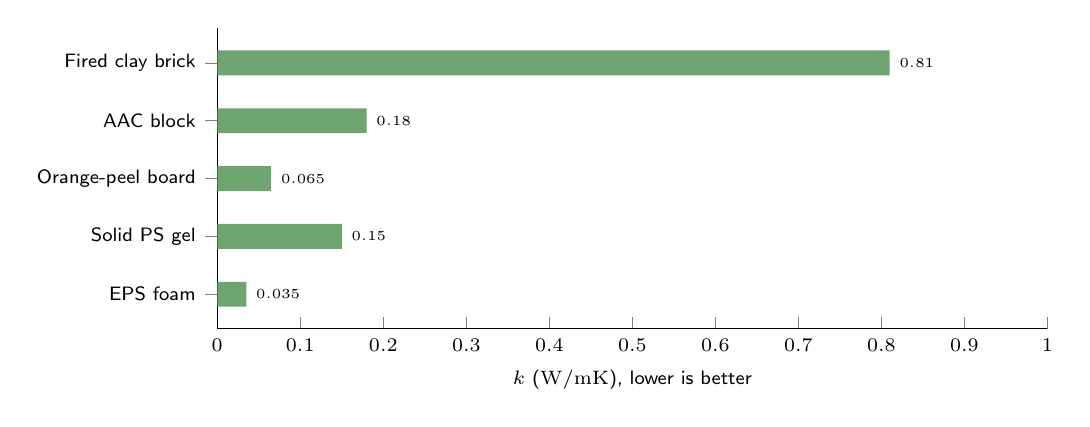
\begin{tikzpicture}
\begin{axis}[
  xbar, width=\linewidth, height=5.4cm, bar width=9pt,
  xmin=0, xmax=1.0, xlabel={$k$ (\si{W/mK}), lower is better},
  xlabel style={font=\scriptsize}, xticklabel style={font=\scriptsize,/pgf/number format/fixed},
  symbolic y coords={EPS foam,Solid PS gel,Orange-peel board,AAC block,Fired clay brick},
  ytick=data, yticklabel style={font=\scriptsize},
  nodes near coords, nodes near coords style={font=\tiny,/pgf/number format/fixed,/pgf/number format/precision=3},
  axis lines*=left, enlarge y limits=0.15]
\addplot[fill=leaf!70,draw=none] coordinates
  {(0.035,EPS foam) (0.15,Solid PS gel) (0.065,Orange-peel board) (0.18,AAC block) (0.81,Fired clay brick)};
\end{axis}
\end{tikzpicture}
\captionof{figure}{Thermal conductivity of wall materials (typical values).}
\end{minipage}

The CoolBrick puts that principle into one block. Figure~\ref{fig:xsec} shows the layers from the sunny outside face to the room side.

\begin{figure}[H]
\centering
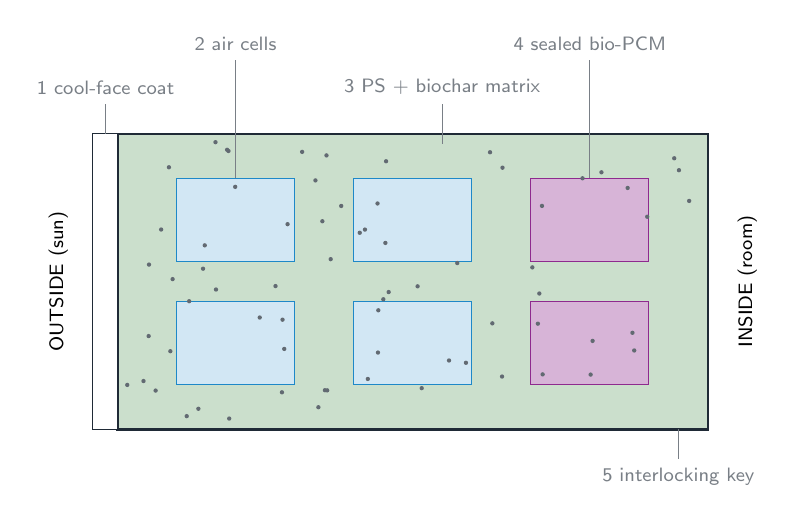
\begin{tikzpicture}[scale=1.25]
  \fill[leaf!25] (0,0) rectangle (6,3);
  \draw[ink,line width=1pt] (0,0) rectangle (6,3);
  \fill[white] (-0.25,0) rectangle (0,3); \draw[ink] (-0.25,0) rectangle (0,3);
  \foreach \x in {0.6,2.4}{\fill[sky!20] (\x,0.45) rectangle ++(1.2,0.85); \draw[sky] (\x,0.45) rectangle ++(1.2,0.85);
                           \fill[sky!20] (\x,1.7) rectangle ++(1.2,0.85); \draw[sky] (\x,1.7) rectangle ++(1.2,0.85);}
  \fill[plum!35] (4.2,0.45) rectangle ++(1.2,0.85); \draw[plum] (4.2,0.45) rectangle ++(1.2,0.85);
  \fill[plum!35] (4.2,1.7) rectangle ++(1.2,0.85); \draw[plum] (4.2,1.7) rectangle ++(1.2,0.85);
  \pgfmathsetseed{7}
  \foreach \i in {1,...,70}{\fill[ink!70] ({0.1+5.8*rnd},{0.08+2.84*rnd}) circle (0.022);}
  \node[font=\scriptsize,rotate=90] at (-0.6,1.5) {OUTSIDE (sun)};
  \node[font=\scriptsize,rotate=90] at (6.4,1.5) {INSIDE (room)};
  \draw[ink!60] (-0.12,3) -- (-0.12,3.3) node[above,font=\scriptsize]{1 cool-face coat};
  \draw[ink!60] (1.2,2.55) -- (1.2,3.75) node[above,font=\scriptsize]{2 air cells};
  \draw[ink!60] (3.3,2.9) -- (3.3,3.3) node[above,font=\scriptsize]{3 PS + biochar matrix};
  \draw[ink!60] (4.8,2.55) -- (4.8,3.75) node[above,font=\scriptsize]{4 sealed bio-PCM};
  \draw[ink!60] (5.7,0) -- (5.7,-0.3) node[below,font=\scriptsize]{5 interlocking key};
\end{tikzpicture}
\caption{Cross-section concept of a CoolBrick, from outside (left) to inside (right).}\label{fig:xsec}
\end{figure}

\subsection{The five cooling upgrades}
\begin{figure}[htbp]
\centering
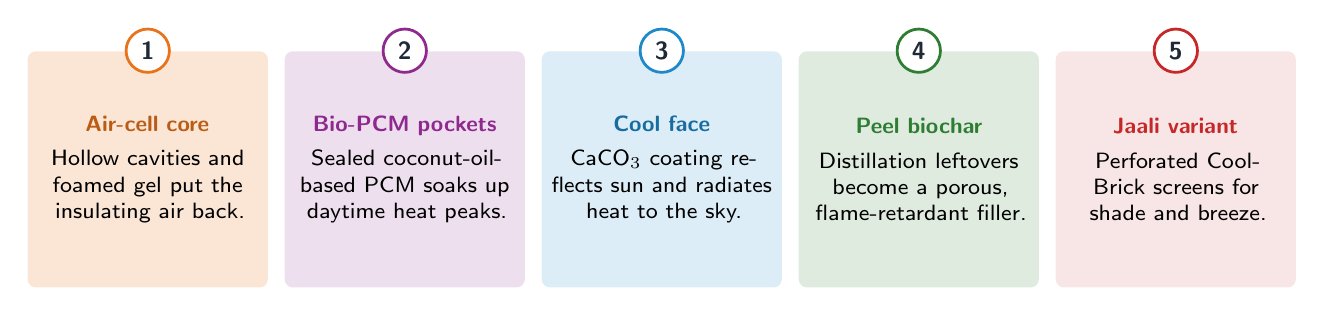
\begin{tikzpicture}[
  feat/.style={rectangle,rounded corners=3pt,minimum width=3.05cm,minimum height=3.0cm,
               text width=2.8cm,align=center,font=\footnotesize,draw=none},
  num/.style={circle,fill=white,text=ink,font=\small\bfseries,inner sep=1pt,minimum size=0.55cm}]
\node[feat,fill=citrus!18] (f1) {\textbf{\color{citrus!80!black}Air-cell core}\\[3pt]Hollow cavities and foamed gel put the insulating air back.};
\node[feat,fill=plum!15,right=0.2cm of f1] (f2) {\textbf{\color{plum}Bio-PCM pockets}\\[3pt]Sealed coconut-oil-based PCM soaks up daytime heat peaks.};
\node[feat,fill=sky!15,right=0.2cm of f2] (f3) {\textbf{\color{sky!80!black}Cool face}\\[3pt]CaCO$_3$ coating reflects sun and radiates heat to the sky.};
\node[feat,fill=leaf!15,right=0.2cm of f3] (f4) {\textbf{\color{leaf}Peel biochar}\\[3pt]Distillation leftovers become a porous, flame-retardant filler.};
\node[feat,fill=heat!12,right=0.2cm of f4] (f5) {\textbf{\color{heat}Jaali variant}\\[3pt]Perforated CoolBrick screens for shade and breeze.};
\foreach \i/\c in {1/citrus,2/plum,3/sky,4/leaf,5/heat}{\node[num,draw=\c,line width=1pt] at (f\i.north) {\i};}
\end{tikzpicture}
\caption{Overview of the five upgrades.}
\end{figure}

\subsubsection*{Upgrade 1 --- Air-cell core}

\begin{minipage}[c]{0.54\textwidth}
\small
\begin{tabular}{@{}lcc@{}}
\toprule
Wall material (230 mm) & $k_\text{eff}$ (\si{W/mK}) & $U$ (\si{W/m^2K}) \\
\midrule
Fired clay brick       & 0.81 & \textbf{2.20} \\
AAC block (benchmark)  & 0.18 & 0.69 \\
Poly Citra v1 (solid)  & 0.20\textsuperscript{*} & 0.76 \\
\textcolor{citrus}{CoolBrick v2 (target)} & \textcolor{citrus}{0.15\textsuperscript{*}} & \textcolor{citrus}{\textbf{0.59}} \\
\bottomrule
\end{tabular}

\footnotesize\textsuperscript{*}Estimates, to be measured with a guarded hot plate (IS 3346).
Example: $U_\text{clay} = 1/(0.13 + 0.23/0.81 + 0.04) = \SI{2.20}{W/m^2K}$.

\small Air is added through (a) moulded hollow cells ($\sim$30--40\% void),
(b) partial foaming of the gel, and (c) porous biochar filler. Result: up to
\textbf{about 73\% less heat conducted} than through fired clay.
\end{minipage}\hfill
\begin{minipage}[c]{0.42\textwidth}
\centering
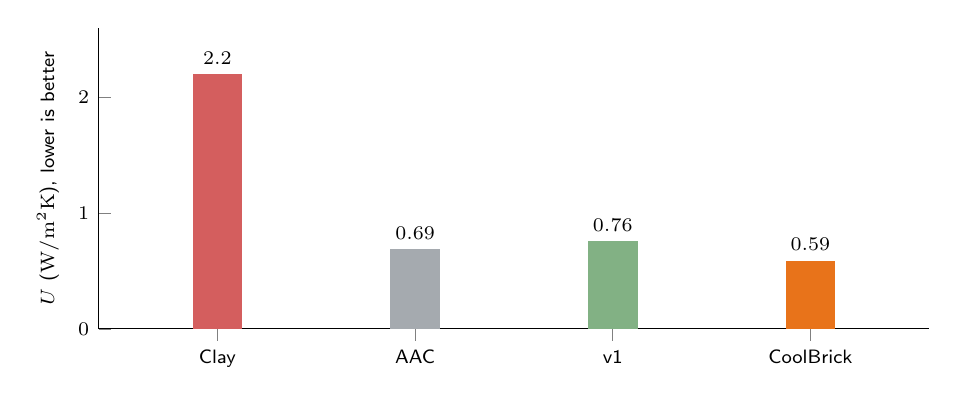
\begin{tikzpicture}
\begin{axis}[
  ybar, width=\linewidth, height=5.4cm, bar width=18pt, bar shift=0pt,
  ymin=0, ymax=2.6, ylabel={$U$ (\si{W/m^2K}), lower is better},
  ylabel style={font=\scriptsize}, yticklabel style={font=\scriptsize},
  symbolic x coords={Clay,AAC,v1,CoolBrick},
  xtick={Clay,AAC,v1,CoolBrick}, xticklabel style={font=\scriptsize},
  nodes near coords, nodes near coords style={font=\scriptsize},
  axis lines*=left, enlarge x limits=0.2]
\addplot[fill=heat!75,draw=none] coordinates {(Clay,2.20)};
\addplot[fill=ink!40,draw=none] coordinates {(AAC,0.69)};
\addplot[fill=leaf!60,draw=none] coordinates {(v1,0.76)};
\addplot[fill=citrus,draw=none] coordinates {(CoolBrick,0.59)};
\end{axis}
\end{tikzpicture}
\captionof{figure}{U-value of a one-brick wall.}
\end{minipage}

\subsubsection*{Upgrade 2 --- Bio-PCM pockets: a thermal battery}

\begin{minipage}[c]{0.5\textwidth}
\small
\begin{itemize}
  \item A \textbf{phase-change material} (PCM) melts when the room passes
        its melting point, absorbing large amounts of heat at near-constant
        temperature, and re-solidifies at night.
  \item Candidate: a \textbf{coconut-oil-based blend}. Pure coconut oil
        melts at about \SI{24}{\celsius}; the blend is tuned to
        \SIrange{26}{28}{\celsius} for Indian comfort.
  \item Sealed in polystyrene cavities, which are water-proof.
        \todo{verify oil--PS compatibility}
  \item In a kennel, the PCM sits on the room side, so the wall next to the
        dog stays close to its melting point through the hottest hours.
  \item Published PCM-brick studies report \textbf{lower peaks (from about
        3 up to about \SI{11}{\celsius}) and time delays of about 2 hours},
        depending on the set-up.
\end{itemize}
\end{minipage}\hfill
\begin{minipage}[c]{0.46\textwidth}
\centering
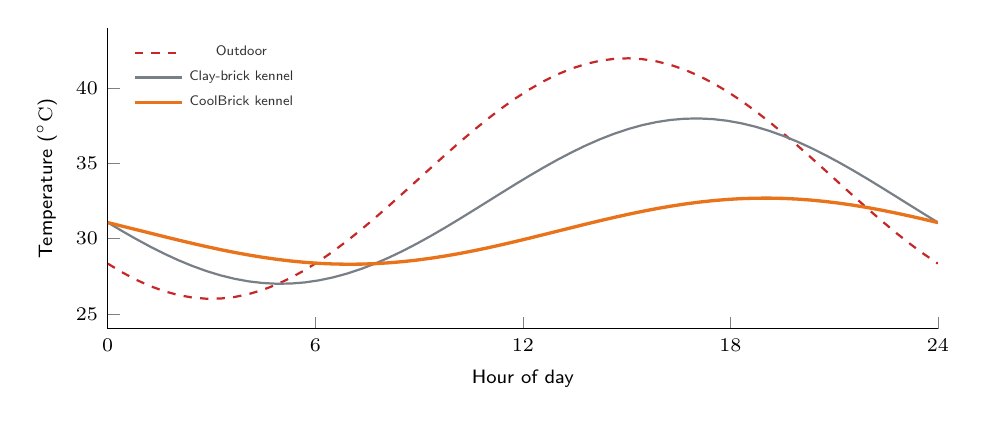
\begin{tikzpicture}
\begin{axis}[
  width=\linewidth, height=5.4cm,
  xmin=0, xmax=24, ymin=24, ymax=44,
  xtick={0,6,12,18,24}, xlabel={Hour of day}, ylabel={Temperature (\si{\celsius})},
  xlabel style={font=\scriptsize}, ylabel style={font=\scriptsize},
  ticklabel style={font=\scriptsize}, axis lines*=left,
  legend style={font=\tiny,at={(0.02,0.98)},anchor=north west,draw=none,fill=white,fill opacity=0.8},
  domain=0:24, samples=60]
\addplot[heat,thick,dashed] {34+8*sin(deg((x-9)*pi/12))};
\addlegendentry{Outdoor}
\addplot[ink!60,thick] {32.5+5.5*sin(deg((x-11)*pi/12))};
\addlegendentry{Clay-brick kennel}
\addplot[citrus,very thick] {30.5+2.2*sin(deg((x-13)*pi/12))};
\addlegendentry{CoolBrick kennel}
\end{axis}
\end{tikzpicture}
\captionof{figure}{Idea of the PCM effect (illustrative only; see Section~5 for simulation results).}
\end{minipage}

\subsubsection*{Upgrade 3 --- The cool face: radiative cooling}

\begin{minipage}[c]{0.56\textwidth}
\small
\begin{itemize}
  \item In direct sun, ordinary walls get much hotter than the air around
        them.
  \item A \textbf{calcium-carbonate radiative-cooling coat} (Purdue
        University, 2020) reflects \textbf{95.5\%} of sunlight and emits heat
        through the atmosphere's ``sky window'' (\SIrange{8}{13}{\micro m},
        emissivity 0.94).
  \item In field tests the surface stayed \textbf{1.7\,\si{\celsius} below
        air temperature at noon} and \SI{10}{\celsius} below at night.
  \item CaCO$_3$ is cheap and can come from \textbf{waste eggshells or marble
        slurry}, giving a third waste stream. A kennel roof gets the
        strongest sun of the day, so it gets this coat first. The coat also shields
        polystyrene from UV damage.
\end{itemize}
\end{minipage}\hfill
\begin{minipage}[c]{0.4\textwidth}
\centering
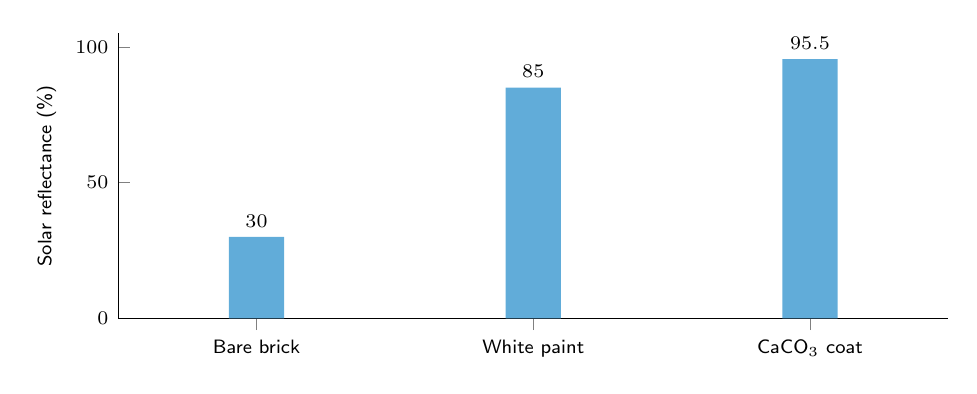
\begin{tikzpicture}
\begin{axis}[
  ybar, width=\linewidth, height=5.2cm, bar width=20pt,
  ymin=0, ymax=105, ylabel={Solar reflectance (\%)},
  ylabel style={font=\scriptsize}, yticklabel style={font=\scriptsize},
  symbolic x coords={Bare brick,White paint,CaCO$_3$ coat},
  xtick=data, xticklabel style={font=\scriptsize},
  nodes near coords, nodes near coords style={font=\scriptsize},
  axis lines*=left, enlarge x limits=0.25]
\addplot[fill=sky!70,draw=none] coordinates {(Bare brick,30) (White paint,85) (CaCO$_3$ coat,95.5)};
\end{axis}
\end{tikzpicture}
\captionof{figure}{Solar reflectance of wall finishes (typical values).}
\end{minipage}

\subsubsection*{Upgrade 4 --- Peel biochar: using the whole orange}

\begin{minipage}[c]{0.54\textwidth}
\small
After steam distillation, the peel residue is still waste. We
\textbf{pyrolyse it into biochar} and mix it into the gel:
\begin{itemize}
  \item \textbf{Porous:} adds trapped air and lowers $k$. Orange-peel
        biochar in a polymer composite reached $k = \SI{0.081}{W/mK}$.
  \item \textbf{Flame-retardant:} the same study achieved a UL-94
        \textbf{V-1} rating. This tackles the biggest weakness of any
        polystyrene product: \textcolor{heat}{fire}.
  \item \textbf{Stores carbon:} biochar locks carbon into the wall instead
        of releasing it when peels are burned.
\end{itemize}
\end{minipage}\hfill
\begin{minipage}[c]{0.42\textwidth}
\centering
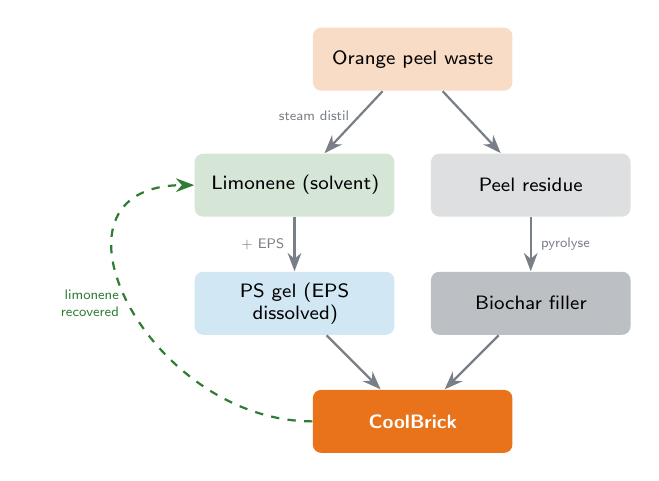
\begin{tikzpicture}[
  n/.style={rectangle,rounded corners=3pt,text width=2.3cm,align=center,font=\scriptsize,minimum height=0.8cm},
  a/.style={-{Stealth},thick,ink!60}]
\node[n,fill=citrus!25] (p) at (2.1,4.6) {Orange peel waste};
\node[n,fill=leaf!20] (l) at (0.6,3.0) {Limonene (solvent)};
\node[n,fill=ink!15] (r) at (3.6,3.0) {Peel residue};
\node[n,fill=sky!20] (g) at (0.6,1.5) {PS gel (EPS dissolved)};
\node[n,fill=ink!30] (b) at (3.6,1.5) {Biochar filler};
\node[n,fill=citrus,text=white] (c) at (2.1,0) {\textbf{CoolBrick}};
\draw[a] (p) -- node[left,font=\tiny,pos=0.4]{steam distil} (l);
\draw[a] (p) -- (r);
\draw[a] (r) -- node[right,font=\tiny]{pyrolyse} (b);
\draw[a] (l) -- node[left,font=\tiny]{+ EPS} (g);
\draw[a] (g) -- (c); \draw[a] (b) -- (c);
\draw[a,leaf,dashed] (c.west) to[out=180,in=180,looseness=1.6] node[left,font=\tiny,text=leaf,align=right,pos=0.5]{limonene\\recovered} (l.west);
\end{tikzpicture}
\captionof{figure}{Zero-waste use of the orange.}
\end{minipage}

\subsubsection*{Upgrade 5 --- Breeze-block (jaali) CoolBricks}

\begin{minipage}[c]{0.56\textwidth}
\small
\begin{itemize}
  \item Traditional Indian \textbf{jaali} screens shade walls and windows
        while letting breezes through, giving cooling with zero energy.
  \item The gel can be moulded, so the same process can cast
        \textbf{perforated CoolBrick screens} as vent blocks high in the kennel
        wall, so hot air can escape while the dog stays shaded.
  \item In our simulation, good ventilation was essential: without it, the
        dog's own body heat builds up inside a well-insulated kennel.
  \item For hot-dry regions, \textbf{terracotta-clad} panels are an option:
        wet clay surfaces add evaporative cooling.
\end{itemize}
\end{minipage}\hfill
\begin{minipage}[c]{0.4\textwidth}
\centering
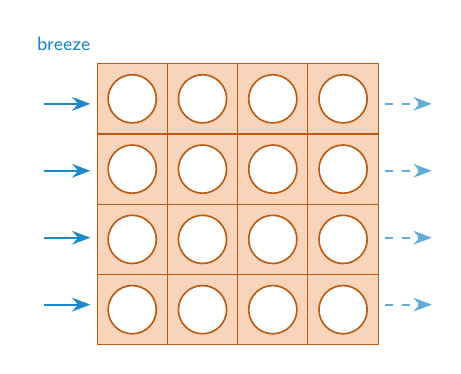
\begin{tikzpicture}[scale=0.85]
  \fill[citrus!30] (0,0) rectangle (4.2,4.2);
  \foreach \x in {0,1.05,2.1,3.15}{\foreach \y in {0,1.05,2.1,3.15}{
     \fill[white] (\x+0.525,\y+0.525) circle (0.36);
     \draw[citrus!80!black,line width=0.6pt] (\x+0.525,\y+0.525) circle (0.36);
     \draw[citrus!80!black,line width=0.4pt] (\x,\y) rectangle ++(1.05,1.05);}}
  \foreach \y in {0.6,1.6,2.6,3.6}{\draw[-{Stealth},sky,thick] (-0.8,\y)--(-0.1,\y);
                                    \draw[-{Stealth},sky!70,thick,dashed] (4.3,\y)--(5.0,\y);}
  \node[font=\scriptsize,sky] at (-0.5,4.5) {breeze};
\end{tikzpicture}
\captionof{figure}{CoolBrick jaali module (concept).}
\end{minipage}

\subsection{The CoolBrick kennel}
\begin{figure}[H]
\centering
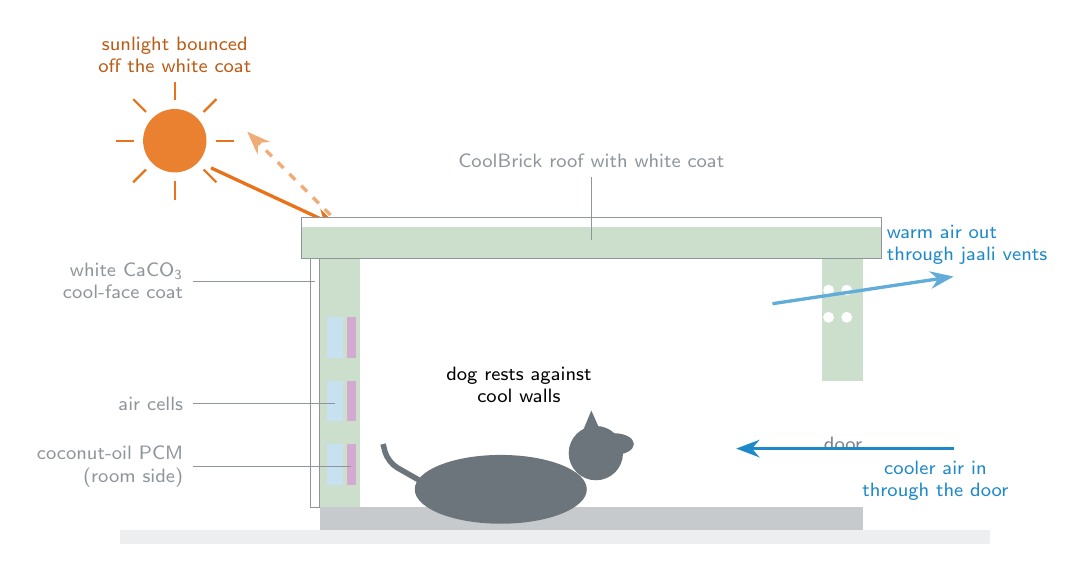
\begin{tikzpicture}[scale=1.15]
  % ground
  \fill[ink!8] (-1.2,-0.15) rectangle (8.4,0);
  % sun
  \fill[citrus!90] (-0.6,4.3) circle (0.35);
  \foreach \a in {0,45,...,315}{\draw[citrus,line width=0.8pt] ($(-0.6,4.3)+(\a:0.45)$)--($(-0.6,4.3)+(\a:0.65)$);}
  \draw[-{Stealth},citrus,line width=1.2pt] (-0.2,4.0)--(1.2,3.35); \draw[-{Stealth},citrus!60,line width=1.2pt,dashed] (1.25,3.35)--(0.2,4.4);
  \node[font=\scriptsize,text=citrus!80!black,align=center] at (-0.6,5.25) {sunlight bounced\\off the white coat};
  % raised floor
  \fill[ink!25] (1.0,0) rectangle (7.0,0.25);
  % walls (CoolBrick)
  \fill[leaf!25] (1.0,0.25) rectangle (1.45,3.0); \fill[leaf!25] (6.55,1.65) rectangle (7.0,3.0); \node[font=\scriptsize,text=ink!60] at (6.78,0.95) {door};
  \fill[white] (0.9,0.25) rectangle (1.0,3.0); \draw[ink!50] (0.9,0.25) rectangle (1.0,3.0);
  \foreach \y in {0.5,1.2,1.9}{\fill[sky!25] (1.08,\y) rectangle ++(0.18,0.45); \fill[plum!40] (1.3,\y) rectangle ++(0.1,0.45);}
  % roof
  \fill[leaf!25] (0.8,3.0) rectangle (7.2,3.35); \fill[white] (0.8,3.35) rectangle (7.2,3.45); \draw[ink!50] (0.8,3.0) rectangle (7.2,3.45);
  % jaali vents
  \foreach \x in {6.62,6.82}{\foreach \y in {2.35,2.65}{\fill[white] (\x,\y) circle (0.06);}}
  \draw[-{Stealth},sky,line width=1.2pt] (8.0,0.9)--(5.6,0.9); \node[font=\scriptsize,text=sky,align=center] at (7.8,0.55) {cooler air in\\through the door};
  \draw[-{Stealth},sky!70,line width=1.2pt] (6.0,2.5)--(8.0,2.8); \node[font=\scriptsize,text=sky,align=left] at (8.15,3.15) {warm air out\\through jaali vents};
  % dog (simple shapes)
  \fill[ink!65] (3.0,0.45) ellipse (0.95 and 0.38);
  \fill[ink!65] (4.05,0.85) circle (0.3);
  \fill[ink!65] (4.25,0.95) ellipse (0.22 and 0.12);
  \fill[ink!65] (3.9,1.08) -- (4.0,1.32) -- (4.12,1.05) -- cycle;
  \draw[ink!65,line width=2pt,rounded corners] (2.1,0.55) -- (1.75,0.75) -- (1.7,0.95);
  \node[font=\scriptsize,align=center] at (3.2,1.6) {dog rests against\\cool walls};
  % labels
  \draw[ink!50] (0.95,2.75)--(-0.4,2.75) node[left,font=\scriptsize,align=right]{white CaCO\textsubscript{3}\\cool-face coat};
  \draw[ink!50] (1.17,1.4)--(-0.4,1.4) node[left,font=\scriptsize]{air cells};
  \draw[ink!50] (1.35,0.7)--(-0.4,0.7) node[left,font=\scriptsize,align=right]{coconut-oil PCM\\(room side)};
  \draw[ink!50] (4.0,3.2)--(4.0,3.9) node[above,font=\scriptsize]{CoolBrick roof with white coat};
\end{tikzpicture}
\caption{How a CoolBrick kennel keeps a dog cool (concept, side view, not to scale).}
\end{figure}

\begin{card}{leaf}
\textbf{Design rule from our simulation:} insulation and ventilation must go
together. A sealed, well-insulated kennel traps the dog's own body heat at
night. Jaali vent blocks high in the walls let warm air out while the door
lets cooler air in.
\end{card}


% =====================================================================
\section{Methodology \& Experimental Design}

\subsection{Making the brick}
\begin{enumerate}
  \item \textbf{Collect} clean Styrofoam packaging and orange peels.
  \item \textbf{Extract D-limonene} from the peels by steam distillation and
        separate the oil from the water.
  \item \textbf{Dissolve} broken Styrofoam in the limonene until it forms a
        thick polystyrene gel \todo{ratio of foam to limonene used}.
  \item \textbf{Mix} in sand or fly ash and the orange-peel biochar
        \todo{mix proportions}.
  \item \textbf{Mould} the gel into brick moulds that form the hollow air
        cells and the PCM pockets. Fill the pockets with the coconut-oil
        blend and seal them.
  \item \textbf{Cure} the bricks under a cover with a simple condenser to
        recover the limonene \todo{curing time and temperature}. Bricks must
        be fully cured so that no citrus solvent is left: concentrated citrus
        oils can irritate dogs.
  \item \textbf{Coat} the outside face with the calcium-carbonate cool-face
        paint, and plaster or seal the inside face.
\end{enumerate}

\begin{figure}[htbp]
\centering
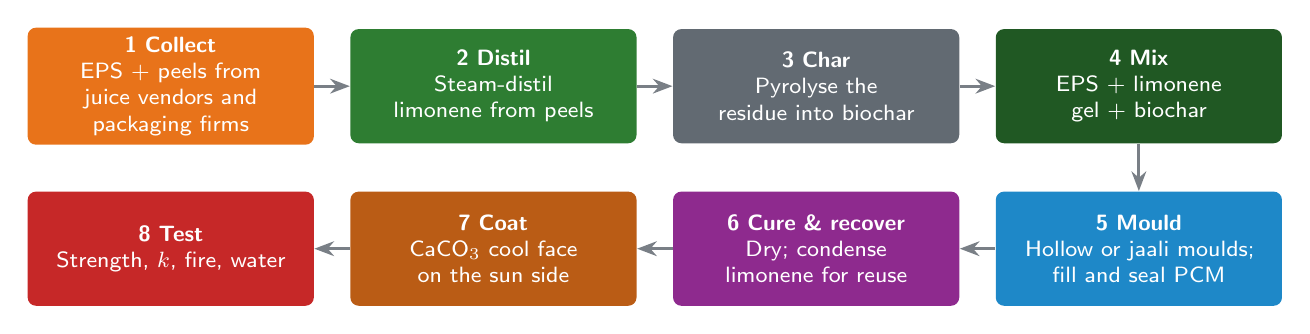
\begin{tikzpicture}[
  s/.style={rectangle,rounded corners=3pt,minimum width=3.6cm,minimum height=1.45cm,
            text width=3.4cm,align=center,font=\footnotesize,text=white},
  arr/.style={-{Stealth[length=2.5mm]},line width=1pt,color=ink!60}]
\node[s,fill=citrus] (1) {\textbf{1 Collect}\\EPS + peels from juice vendors and packaging firms};
\node[s,fill=leaf,right=0.45cm of 1] (2) {\textbf{2 Distil}\\Steam-distil limonene from peels};
\node[s,fill=ink!70,right=0.45cm of 2] (3) {\textbf{3 Char}\\Pyrolyse the residue into biochar};
\node[s,fill=leaf!70!black,right=0.45cm of 3] (4) {\textbf{4 Mix}\\EPS + limonene gel + biochar};
\node[s,fill=sky,below=0.6cm of 4] (5) {\textbf{5 Mould}\\Hollow or jaali moulds; fill and seal PCM};
\node[s,fill=plum,left=0.45cm of 5] (6) {\textbf{6 Cure \& recover}\\Dry; condense limonene for reuse};
\node[s,fill=citrus!80!black,left=0.45cm of 6] (7) {\textbf{7 Coat}\\CaCO$_3$ cool face on the sun side};
\node[s,fill=heat,left=0.45cm of 7] (8) {\textbf{8 Test}\\Strength, $k$, fire, water};
\foreach \a/\b in {1/2,2/3,3/4,4/5,5/6,6/7,7/8}{\draw[arr] (\a)--(\b);}
\end{tikzpicture}
\caption{Version 2 production process with closed solvent loop.}
\end{figure}

\begin{card}{leaf}
\textbf{Closed solvent loop:} curing in a covered tray with a simple
condenser recovers the limonene vapour instead of releasing it, which
lowers cost, odour and VOC emissions.
\end{card}


\subsection{Experimental design}
\textbf{Aim:} to find out whether a CoolBrick kennel stays cooler inside than a
clay-brick kennel and a plastic kennel on a hot, sunny day.

\textbf{Hypothesis:} the inside of the CoolBrick kennel will stay at or below
the outdoor air temperature, at least \SI{3}{\celsius} cooler at peak than
the clay and plastic kennels.

\textbf{Ethics:} no animals are used in our tests. A ``dog dummy'' gives off
the same heat as a resting dog. Only after the design is proven would we
place kennels at an animal shelter, where dogs can choose freely whether to
use them, with shelter staff and a vet watching.

\begin{center}
\small
\begin{tabularx}{\textwidth}{@{}>{\bfseries}l X@{}}
\toprule
Independent variable & Kennel material: fired clay brick, plastic kennel, CoolBrick. \\
Dependent variables & Air temperature inside; inner wall and roof surface temperatures; ``felt'' (black-globe) temperature next to the dummy; number of hours above \SI{35}{\celsius}. \\
Control variables & Kennel size (\SI{1.0}{m} $\times$ \SI{0.8}{m} $\times$ \SI{0.8}{m}), door and vent sizes, position and direction in the sun, the same dog dummy, same sensors and logging interval, same days. \\
Dog dummy & A \SI{50}{W} heater inside a water-filled container wrapped in an old blanket, about the size and heat output of a resting medium-sized dog. \\
Equipment & Three model kennels, three dog dummies, Arduino with DS18B20 temperature sensors, black-globe thermometers, IR thermometer. \\
Repeats & 30 summer days; each brick test on at least 5 bricks. \\
\bottomrule
\end{tabularx}
\end{center}

\subsection{Tests on the brick}
\begin{center}
\small
\begin{tabularx}{\textwidth}{@{}l X l l@{}}
\toprule
\textbf{Property} & \textbf{Method} & \textbf{Standard} & \textbf{Target} \\
\midrule
Compressive strength & Universal testing machine, 5 samples per mix & IS 3495 (Pt 1) & $\geq$ \SI{3.5}{MPa} \\
Water absorption     & 24 h immersion, weigh before and after & IS 3495 (Pt 2) & $<$ 5\% \\
Thermal conductivity & Guarded hot plate (or DIY hot-box) & IS 3346 & $k \leq$ \SI{0.15}{W/mK} \\
Fire behaviour       & Bunsen-flame burn test: char length, dripping & UL-94 (adapted) & V-1 or better \\
PCM performance      & DSC (melting point, latent heat) at a partner lab & --- & about \SI{27}{\celsius} \\
Surface temperature  & IR thermometer, coated vs.\ uncoated at noon & --- & $\leq$ air temp. \\
Leftover solvent     & Weigh during curing until steady; smell test & --- & no citrus smell \\
\bottomrule
\end{tabularx}
\end{center}

\subsection{Computer simulation}
Before building, we tested the kennel with a computer model that we wrote
in JavaScript. Each wall is split into thin slices. Every 5 seconds of
simulated time the program calculates how much heat moves between
neighbouring slices using Fourier's law, $q = k\,\Delta T/\Delta x$. On the
outside, each wall and the roof absorb sunlight ($\alpha I$), exchange heat
with the air ($h_o = \SI{15}{W/m^2K}$) and radiate heat to a sky about
\SI{18}{\celsius} colder than the air (Stefan--Boltzmann law). Inside, the
air gains \SI{50}{W} from the resting dog and heat from the walls
($h_i = \SI{8}{W/m^2K}$), and swaps air with outside through the door and
jaali vents (100 air changes per hour). The ``felt'' temperature is the
average of the inside air and the inside wall surfaces. The weather is a hot
north-Indian day (air 27--\SI{41}{\celsius}, strong sun), run for three days
with the third day reported.

\begin{center}
\small
\begin{tabular}{@{}lccccc@{}}
\toprule
Kennel & Wall & $k$ (W/mK) & $U$ (W/m\textsuperscript{2}K) & Sun absorbed & PCM \\
\midrule
Clay brick & 110 mm fired clay & 0.81 & 3.27 & 70\% & none \\
Plastic & 5 mm polyethylene & 0.40 & 5.48 & 60\% & none \\
CoolBrick & 110 mm CoolBrick & 0.15 / 0.18 & 1.15 & 5\% & 30 mm, melts \SI{27}{\celsius} \\
\bottomrule
\end{tabular}
\end{center}
{\footnotesize\color{gray} CoolBrick values are design targets to be measured. Each kennel uses the same material for walls and roof.}

\subsection{Safety and risks}
\begin{center}
\small
\begin{tabularx}{\textwidth}{@{}>{\bfseries}l X X@{}}
\toprule
Risk & Why it matters & Our mitigation \\
\midrule
Leftover limonene & Concentrated citrus oils can irritate dogs. & Cure fully until weight is steady; plaster or seal the inside face; smell test before use. \\
Chewing & Dogs chew things. & PCM pockets are sealed inside the brick; inside face plastered; coconut oil is non-toxic. \\
Fire & Polystyrene burns and drips. & Biochar filler (V-1 in literature); mineral coat and plaster; burn tests; keep away from cooking fires. \\
UV ageing & Polystyrene yellows and turns brittle in the sun. & CaCO\textsubscript{3} coat or plaster blocks UV on exposed faces. \\
Trapped heat & A sealed, insulated kennel traps the dog's own heat. & Jaali vents high up plus an open door; tested in the simulation. \\
Hygiene & Kennels must be cleaned often. & Waterproof surfaces; raised floor so water drains. \\
Cost & Must be affordable for shelters. & Full cost price analysis and cost-cutting plan (Section~7). \\
\bottomrule
\end{tabularx}
\end{center}


% =====================================================================
\section{Results So Far and Explanation of Results}

\subsection{Prototype results (version 1)}
\begin{figure}[H]
\centering
\begin{subfigure}{0.32\textwidth}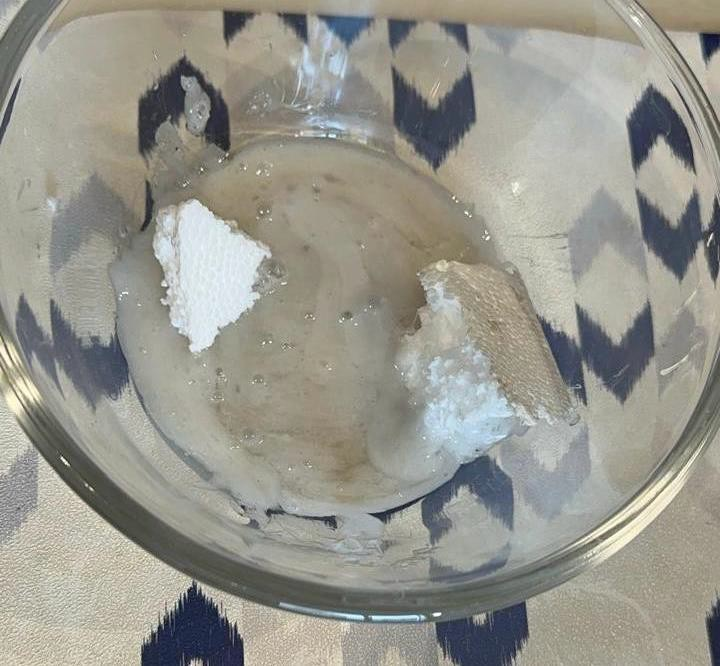
\includegraphics[width=\linewidth,height=3.4cm,keepaspectratio=false]{dissolving.jpg}\caption{Styrofoam dissolving}\end{subfigure}\hfill
\begin{subfigure}{0.32\textwidth}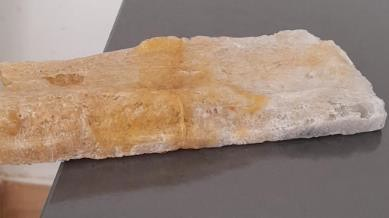
\includegraphics[width=\linewidth,height=3.4cm,keepaspectratio=false]{brick-sample.jpg}\caption{Cured brick sample}\end{subfigure}\hfill
\begin{subfigure}{0.32\textwidth}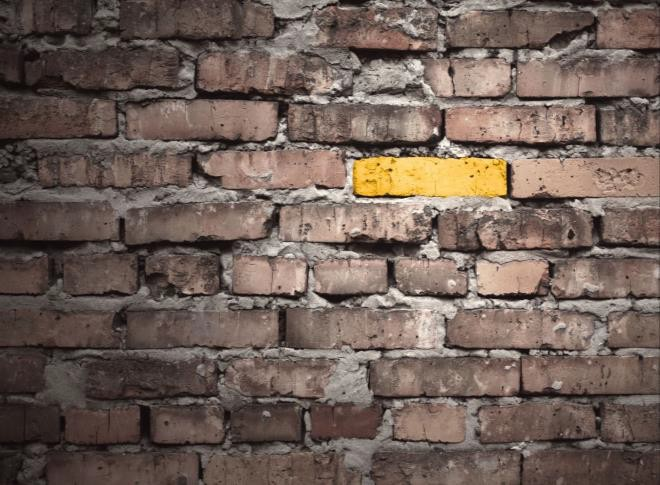
\includegraphics[width=\linewidth,height=3.4cm,keepaspectratio=false]{brickwall.jpg}\caption{Compared with a clay wall}\end{subfigure}\\[6pt]
\begin{subfigure}{0.32\textwidth}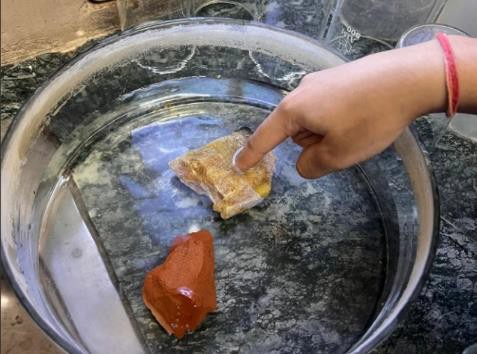
\includegraphics[width=\linewidth,height=3.4cm,keepaspectratio=false]{water-test.jpg}\caption{Water test}\end{subfigure}\hfill
\begin{subfigure}{0.32\textwidth}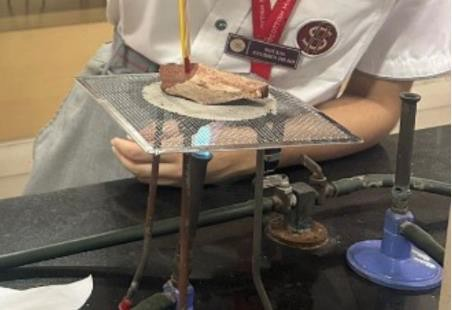
\includegraphics[width=\linewidth,height=3.4cm,keepaspectratio=false]{heat-test.jpg}\caption{Heat test}\end{subfigure}\hfill
\begin{subfigure}{0.32\textwidth}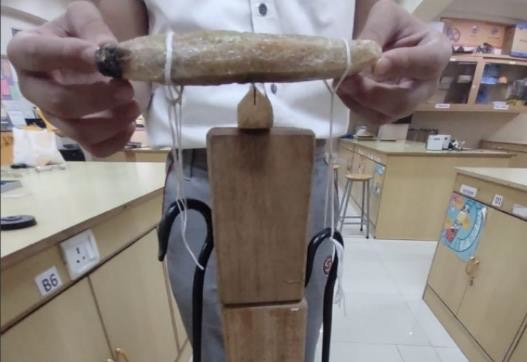
\includegraphics[width=\linewidth,height=3.4cm,keepaspectratio=false]{load-test.jpg}\caption{Load test}\end{subfigure}
\caption{Making and testing the Poly Citra Brick prototype.}
\end{figure}

We have made and tested Poly Citra v1 bricks. They float in water, show
little water absorption, keep their shape when heated and hold a load
\todo{add the measured values: mass, density, water absorption, load held,
heat test temperature}.

\subsection{Simulation results: the CoolBrick kennel}

\begin{figure}[H]
\centering
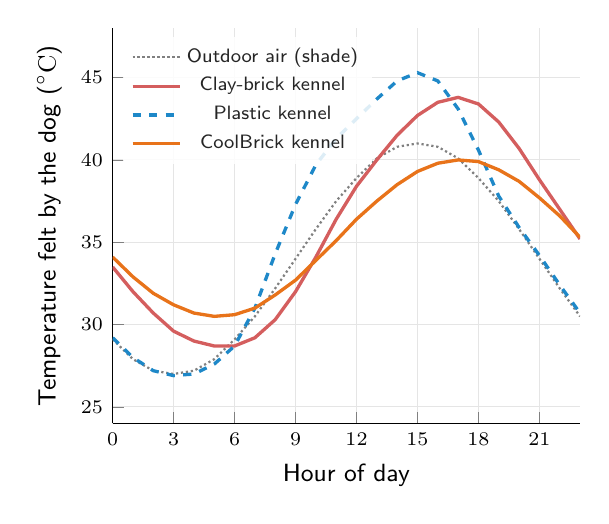
\begin{tikzpicture}
\begin{axis}[width=0.62\textwidth,height=6.6cm,xmin=0,xmax=23,ymin=24,ymax=48,xtick={0,3,6,9,12,15,18,21},
  xlabel={Hour of day},ylabel={Temperature felt by the dog (\si{\celsius})},label style={font=\small},tick label style={font=\scriptsize},
  legend style={font=\scriptsize,at={(0.02,0.98)},anchor=north west,draw=none,fill=white,fill opacity=0.85},grid=major,grid style={gray!20},axis lines*=left]
\addplot[gray,thick,densely dotted] coordinates {(0,29.1) (1,27.9) (2,27.2) (3,27) (4,27.2) (5,27.9) (6,29.1) (7,30.5) (8,32.2) (9,34) (10,35.8) (11,37.5) (12,38.9) (13,40.1) (14,40.8) (15,41) (16,40.8) (17,40.1) (18,38.9) (19,37.5) (20,35.8) (21,34) (22,32.2) (23,30.5)};
\addlegendentry{Outdoor air (shade)}
\addplot[heat!75,very thick] coordinates {(0,33.5) (1,32) (2,30.7) (3,29.6) (4,29) (5,28.7) (6,28.7) (7,29.2) (8,30.3) (9,32) (10,34.1) (11,36.4) (12,38.4) (13,40) (14,41.5) (15,42.7) (16,43.5) (17,43.8) (18,43.4) (19,42.3) (20,40.7) (21,38.8) (22,37) (23,35.2)};
\addlegendentry{Clay-brick kennel}
\addplot[sky,very thick,dashed] coordinates {(0,29.2) (1,28) (2,27.2) (3,26.9) (4,27) (5,27.6) (6,28.7) (7,31) (8,34.3) (9,37.3) (10,39.7) (11,41.3) (12,42.5) (13,43.7) (14,44.8) (15,45.3) (16,44.8) (17,43.1) (18,40.6) (19,37.8) (20,35.9) (21,34.2) (22,32.4) (23,30.7)};
\addlegendentry{Plastic kennel}
\addplot[citrus,very thick] coordinates {(0,34.1) (1,32.9) (2,31.9) (3,31.2) (4,30.7) (5,30.5) (6,30.6) (7,31) (8,31.8) (9,32.7) (10,33.9) (11,35.1) (12,36.4) (13,37.5) (14,38.5) (15,39.3) (16,39.8) (17,40) (18,39.9) (19,39.4) (20,38.7) (21,37.7) (22,36.6) (23,35.3)};
\addlegendentry{CoolBrick kennel}
\end{axis}
\end{tikzpicture}\hfill
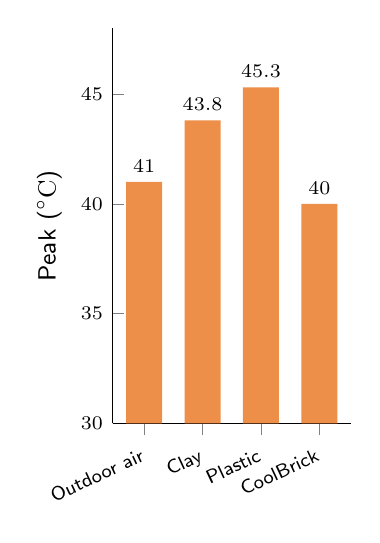
\begin{tikzpicture}
\begin{axis}[ybar,width=0.38\textwidth,height=6.6cm,bar width=13pt,ymin=30,ymax=48,
  symbolic x coords={Outdoor air,Clay,Plastic,CoolBrick},xtick=data,x tick label style={font=\scriptsize,rotate=25,anchor=north east},
  nodes near coords,nodes near coords style={font=\scriptsize},
  ylabel={Peak (\si{\celsius})},label style={font=\small},tick label style={font=\scriptsize},axis lines*=left,enlarge x limits=0.18]
\addplot[fill=citrus!80,draw=none] coordinates {(Outdoor air,41.0) (Clay,43.8) (Plastic,45.3) (CoolBrick,40.0)};
\end{axis}
\end{tikzpicture}
\caption{Simulated temperature felt by a resting dog inside each kennel on a hot day. Left: through the day. Right: the hottest point.}
\end{figure}

\begin{center}
\small
\begin{tabular}{@{}lccc@{}}
\toprule
Simulation result & Clay brick & Plastic & CoolBrick \\
\midrule
Wall U-value (W/m\textsuperscript{2}K) & 3.27 & 5.48 & 1.15 \\
Hottest ``felt'' temperature (\si{\celsius}) & 43.8 & 45.3 & 40.0 \\
Hottest inside air (\si{\celsius}) & 43.5 & 45.3 & 40.8 \\
Hottest inside wall surface (\si{\celsius}) & 44.2 & 45.4 & 39.5 \\
Hours above \SI{35}{\celsius} (``felt'') & 12.7 & 12.3 & 12.3 \\
\bottomrule
\end{tabular}
\end{center}
{\footnotesize\color{gray} For comparison, the outdoor air in the shade peaks at \SI{41}{\celsius} and is above \SI{35}{\celsius} for 10.8 hours.}

\subsection{Explanation of the results}
\begin{itemize}
  \item \textbf{Clay and plastic kennels get hotter than the air outside.}
        They absorb most of the sunlight, so their walls and roof heat up
        and radiate that heat onto the dog. At the hottest point the dog
        feels about 43.8 and 45.3 \si{\celsius}, which is
        2.8--4.3 \si{\celsius} hotter than resting in
        the shade.
  \item \textbf{The CoolBrick kennel stays below the outdoor air.} The white
        coat reflects about 95\% of sunlight, the air cells slow the heat
        that does get in, and the PCM soaks up the rest. The inside walls
        peak at about 39.5 \si{\celsius}, about
        4.7 \si{\celsius} cooler than the clay kennel's walls.
  \item \textbf{Ventilation matters as much as insulation.} When we first ran
        the model with less ventilation, the well-insulated CoolBrick kennel
        trapped the dog's own heat at night. Adding jaali vents (about 100
        air changes per hour) fixed this. This is now a design rule.
  \item \textbf{Limits.} No kennel can be cooler than the outside air for
        long without a power source, so on a \SI{41}{\celsius} day all three
        stay hot for many hours. The CoolBrick's job is to stop the kennel
        from making things \emph{worse} than the shade. These are model
        results with assumed values; real kennels will have mortar joints
        and imperfections. The dog-dummy experiment will test this.
\end{itemize}

\subsection{Measured results (to be completed) \todo{fill in}}
\begin{center}
\small
\begin{tabular}{@{}lccc@{}}
\toprule
 & Clay brick & Plastic & CoolBrick \\
\midrule
Mass per brick (kg)                       & \todo{} & --- & \todo{} \\
Compressive strength (MPa)                & \todo{} & --- & \todo{} \\
Water absorption (\%)                     & \todo{} & --- & \todo{} \\
Outer surface temperature at noon (\si{\celsius}) & \todo{} & \todo{} & \todo{} \\
Peak ``felt'' temperature in kennel (\si{\celsius}) & \todo{} & \todo{} & \todo{} \\
Hours above \SI{35}{\celsius}            & \todo{} & \todo{} & \todo{} \\
\bottomrule
\end{tabular}
\end{center}


% =====================================================================
\section{Conclusion}

Poly Citra Bricks show that two common wastes, Styrofoam and orange peel, can
be turned into a light, waterproof building brick without mining clay or
firing a kiln. By redesigning the brick to ``put the air back'' and adding a
reflective coat, a coconut-oil PCM and peel biochar, the CoolBrick becomes a
\textbf{passive cooling material}. Our simulation of a dog kennel on a
\SI{41}{\celsius} day predicts that a resting dog would feel about
40.0 \si{\celsius} at the hottest point in a CoolBrick kennel, compared
with 43.8 \si{\celsius} in a clay-brick kennel and 45.3 \si{\celsius} in a plastic one,
with the walls next to the dog about 4.7 \si{\celsius} cooler than clay. This
supports our hypothesis. We also learned that good ventilation is essential.
A CoolBrick kennel costs about \rupee11,059 to make at scale, close to a
plastic kennel, or about \rupee3 per day over a 10-year life. The next
step is to measure the real bricks and run the dog-dummy experiment.

\begin{center}
\small
\begin{tabularx}{\textwidth}{@{}>{\bfseries}l X X@{}}
\toprule
 & Poly Citra Bricks (v1) & Poly Citra CoolBrick (v2) \\
\midrule
Goal & Turn two wastes into a brick & \ldots{} that also \textbf{keeps dogs cool} \\
Audience & NGOs, housing, government & \textbf{Animal shelters}, street-dog carers, pet owners, dog units \\
Inputs & EPS + orange-peel limonene & + peel biochar, coconut-oil PCM, CaCO\textsubscript{3} coat \\
Structure & Solid moulded brick & Hollow air cells, sealed PCM pockets, interlocking key, jaali vent blocks \\
Thermal & Not measured & Kennel stays below outdoor air in simulation; \\
 & & walls \textasciitilde 4.7 \si{\celsius} cooler than clay \\
Cost & Not worked out & \rupee67 per brick, \rupee11,059 per kennel at scale \\
Fire safety & Not addressed & Biochar flame retardance, mineral coat, burn testing \\
Solvent & Single use & Recovered by condensation and reused \\
Evidence & Prototype & Standard tests + 30-day dog-dummy kennel experiment \\
\bottomrule
\end{tabularx}
\end{center}


% =====================================================================
\section{Future Potential of the Project}

\subsection{Cost price analysis}
All prices are 2025--26 Indian market estimates from supplier listings and
are rounded. They will change with location and quantity, so we will get
quotes before building. ``Pilot'' means making about 25 bricks a day by
hand; ``scale'' means about 150 bricks a day per worker with more moulds.

\subsubsection*{A. Cost price of one CoolBrick (23 $\times$ 11 $\times$ 7.5 cm)}
\begin{center}
\small
\begin{tabularx}{\textwidth}{@{}l X r@{}}
\toprule
\textbf{Item} & \textbf{Basis} & \textbf{\rupee per brick} \\
\midrule
Styrofoam (EPS) waste & about 0.49 kg, donated; collection and cleaning & 3.0 \\
D-limonene top-up & 140 g used per brick, 80\% recovered; 28 g lost at \rupee590/kg & 16.5 \\
Sand / fly-ash filler & 0.84 kg at \rupee1.5/kg & 1.3 \\
Orange-peel biochar & 50 g from free peel; fuel for charring & 1.0 \\
Coconut-oil PCM blend & 0.21 L at \rupee160/L (industrial grade) & 33.3 \\
Sealing the PCM pockets & gel caps and tape & 2.0 \\
CaCO\textsubscript{3} cool-face coat & 0.017 m\textsuperscript{2} at about \rupee55/m\textsuperscript{2} & 1.0 \\
Energy & distilling, curing and solvent recovery & 4.0 \\
Mould wear & reusable moulds over about 500 uses & 1.0 \\
\midrule
\textbf{Materials and energy} & & \textbf{63.1} \\
Labour, pilot & 25 bricks a day at \rupee600/day & 24.0 \\
Labour, at scale & 150 bricks a day at \rupee600/day & 4.0 \\
\midrule
\textbf{Cost price, pilot / at scale} & & \textbf{87 / 67} \\
\textbf{``Lite'' brick (no PCM), pilot / at scale} & & \textbf{52 / 32} \\
Fired clay brick, for comparison & market price & 5--12 \\
\bottomrule
\end{tabularx}
\end{center}

\begin{minipage}[t]{0.54\textwidth}
\vspace{0pt}
\textbf{What drives the cost.} The coconut-oil PCM is about half the cost of
a CoolBrick. The limonene top-up is the next biggest, and it depends on how
much solvent we recover:

\begin{center}
\small
\begin{tabular}{@{}lccc@{}}
\toprule
Limonene recovered & 60\% & 80\% & 95\% \\
\midrule
Limonene cost per brick (\rupee) & 33 & 17 & 4 \\
\bottomrule
\end{tabular}
\end{center}
If we distil all our own limonene from free orange peel, this cost becomes
mainly fuel. About 4.7 kg of peel replaces the 28 g lost per brick.
\end{minipage}\hfill
\begin{minipage}[t]{0.42\textwidth}
\vspace{0pt}
\begin{card}{citrus}\textbf{A CoolBrick costs more than a clay brick} (about
\rupee67 vs \rupee5--12). It does much more: it insulates,
reflects sun and stores heat. So we use full CoolBricks only where they
matter most (the roof and the sunny west wall) and cheaper ``Lite'' bricks
elsewhere.\end{card}
\end{minipage}

\subsubsection*{B. Cost of one CoolBrick dog kennel (1.0 $\times$ 0.8 $\times$ 0.8 m)}
The kennel needs about 189 bricks: 140 for the walls (with 5\% spare)
and 49 for the roof. In our ``smart mix'', 82 full CoolBricks go in the
roof and the west wall and 107 Lite bricks go in the other walls.

\begin{center}
\small
\begin{tabular}{@{}lr@{}}
\toprule
\textbf{Item} & \textbf{Cost} \\
\midrule
82 full CoolBricks at \rupee67 (scale) & \rupee5,499 \\
107 Lite bricks at \rupee32 (scale) & \rupee3,400 \\
Fibre-cement sheet to support the roof & \rupee450 \\
Mortar (cement and sand) & \rupee350 \\
Raised floor tiles & \rupee300 \\
Four jaali vent blocks (moulded) & \rupee160 \\
Mason, one day & \rupee900 \\
\midrule
\textbf{Cost price of a CoolBrick kennel, at scale} & \textbf{\rupee11,059} \\
Same kennel at pilot scale & \rupee14,839 \\
All full CoolBricks (no Lite bricks), at scale & \rupee14,834 \\
\bottomrule
\end{tabular}
\end{center}

\begin{figure}[H]
\centering
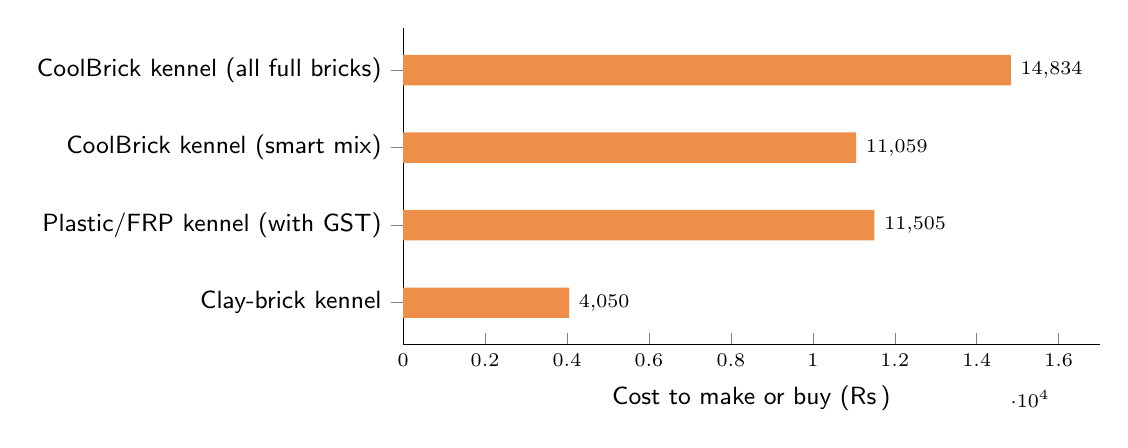
\begin{tikzpicture}
\begin{axis}[xbar,width=0.86\textwidth,height=5.6cm,bar width=11pt,xmin=0,xmax=17000,
  symbolic y coords={A,B,C,D},
  ytick=data,yticklabels={Clay-brick kennel,Plastic/FRP kennel (with GST),CoolBrick kennel (smart mix),CoolBrick kennel (all full bricks)},yticklabel style={font=\small},xticklabel style={font=\scriptsize,/pgf/number format/fixed},
  nodes near coords,nodes near coords style={font=\scriptsize,/pgf/number format/fixed},xlabel={Cost to make or buy (\rupee)},label style={font=\small},axis lines*=left,enlarge y limits=0.18]
\addplot[fill=citrus!80,draw=none] coordinates {(4050,A) (11505,B) (11059,C) (14834,D)};
\end{axis}
\end{tikzpicture}
\caption{Cost of a dog kennel of the same size. The plastic price is one Indian listing for an FRP kennel (\rupee9,750 + 18\% GST, before delivery). The clay kennel uses the same extras as the CoolBrick kennel.}
\end{figure}

\subsubsection*{C. Selling price, profit and break-even}
\begin{center}
\small
\begin{tabular}{@{}lr@{}}
\toprule
Cost price of a CoolBrick kennel (smart mix, at scale) & \rupee11,059 \\
Selling price to shelters and pet owners & \rupee13,500 \\
\textbf{Profit per kennel} & \textbf{\rupee2,441 (22\% of cost)} \\
\midrule
Steam-distillation still and condenser & \rupee12,000 \\
Ten brick moulds & \rupee8,000 \\
Limonene working stock (7 kg) & \rupee4,130 \\
Scale, thermometers, mixing tools & \rupee5,000 \\
\textbf{One-time set-up cost} & \textbf{\rupee29,130} \\
\midrule
\textbf{Break-even} & \textbf{after about 12 kennels} \\
Cost per dog per day over a 10-year life & \rupee3.0 \\
\bottomrule
\end{tabular}
\end{center}

\textbf{How we will bring the cost down:} distil our own limonene from free
peel; buy coconut oil in bulk or test cheaper plant fats for the PCM; make
CaCO\textsubscript{3} coat from waste eggshells; and ask companies to sponsor
kennels for shelters through CSR, so shelters pay little or nothing.

\subsection{Who will use it}
\begin{minipage}[c]{0.62\textwidth}
\begin{itemize}
  \item \textbf{Animal shelters and rescue NGOs}, which house many dogs and
        cannot afford cooling.
  \item \textbf{Municipal Animal Birth Control (ABC) centres}, where dogs
        recover after surgery.
  \item \textbf{Street-dog feeders and resident welfare associations} who
        look after community dogs.
  \item \textbf{Pet owners} whose dogs live outdoors, and farms with guard
        dogs.
  \item \textbf{Police, army and security dog units} with outdoor kennels.
\end{itemize}
\end{minipage}\hfill
\begin{minipage}[c]{0.33\textwidth}
\centering
\includegraphics[width=\linewidth]{audience.png}
\end{minipage}

\subsection{Business model}
\begin{minipage}[c]{0.68\textwidth}
\begin{card}{citrus}\textbf{Kennel kits.} Sell CoolBrick kennel kits and
built kennels to shelters, pet owners and dog units.\end{card}
\begin{card}{leaf}\textbf{Sponsor a CoolKennel.} Companies and donors pay for
kennels placed at shelters through CSR, with a plaque and photos.\end{card}
\begin{card}{sky}\textbf{Partnerships.} Collect Styrofoam from shops and
packaging companies, and peels from juice vendors.\end{card}
\begin{card}{plum}\textbf{Original market.} CoolBricks and Lite bricks for
eco-shelters and housing projects continue alongside.\end{card}
\end{minipage}\hfill
\begin{minipage}[c]{0.28\textwidth}
\centering
\includegraphics[width=\linewidth]{revenue.png}
\end{minipage}

\subsection{Spreading the idea}
\begin{minipage}[c]{0.62\textwidth}
\begin{enumerate}[label=\textcolor{citrus}{\textbf{\arabic*.}}]
  \item \textbf{Kennel demo at a shelter} --- two kennels side by side with
        live temperature displays.
  \item \textbf{Thermal-camera photos} of a CoolBrick kennel vs a plastic one
        at 2\,pm.
  \item \textbf{Social-media stories} of rescued dogs and their cool kennels.
  \item \textbf{Vet and NGO partners} to share heat-safety advice for dogs.
  \item \textbf{Student Ambassador Program} --- youth lead peel and Styrofoam
        collection drives.
\end{enumerate}
\end{minipage}\hfill
\begin{minipage}[c]{0.34\textwidth}
\centering

\includegraphics[width=0.48\linewidth,height=3.6cm,keepaspectratio=false]{social-media.png}\hfill

\includegraphics[width=0.48\linewidth]{ngo.png}
\end{minipage}

\subsection{Roadmap}
\begin{center}
\begin{tikzpicture}[
  ph/.style={rectangle,rounded corners=3pt,minimum width=3.8cm,minimum height=2.8cm,
             text width=3.5cm,align=left,font=\small,anchor=north},
  hd/.style={rectangle,rounded corners=3pt,minimum width=3.8cm,minimum height=0.8cm,
             font=\bfseries,text=white,anchor=south}]
\foreach \i/\c/\t/\b in {
  0/plum/{Now}/{\textbullet\ Brick tests\\\textbullet\ Measure $k$ and strength\\\textbullet\ Check no solvent is left},
  1/sky/{Next 3 months}/{\textbullet\ 30-day dog-dummy kennel trial\\\textbullet\ Tune the PCM blend\\\textbullet\ Coat from eggshells},
  2/leaf/{6 months}/{\textbullet\ 3 pilot kennels at an animal shelter\\\textbullet\ Real cost per kennel},
  3/citrus/{12 months+}/{\textbullet\ Kennel kits\\\textbullet\ CSR sponsors\\\textbullet\ Designs for cats, goats and poultry}}{
  \node[hd,fill=\c] at (\i*4.1,0) {\t};
  \node[ph,fill=\c!10] at (\i*4.1,0) {\b};}
\end{tikzpicture}
\end{center}


% =====================================================================
\section{Bibliography, References and Acknowledgements}

\subsection*{References}
\small
\begin{enumerate}[label={[\arabic*]},leftmargin=*]
\item Department of Animal Husbandry and Dairying (2019). \emph{20th Livestock Census}. Government of India.
\item O'Neill, D.\,G., et al.\ (2020). Heat-related illness in dogs in the UK (VetCompass study). \emph{Scientific Reports}. \todo{complete citation}
\item PetMD (2024). \emph{How Hot Is Too Hot for Dogs?} petmd.com.
\item Li, X., Peoples, J., Huang, Z., Zhao, Z., Qiu, J., \& Ruan, X. (2020).
      Full daytime sub-ambient radiative cooling in commercial-like paints
      with high figure of merit. \emph{Cell Reports Physical Science}, 1(10).
\item Vitale, M., \& Cascone, S. (2022). Orange peels as a potential
      ecological thermal insulation material for building application.
      \emph{TeMA --- Technologies, Engineering, Materials, Architecture}, 8(2).
\item Enhanced biodegradability and thermal insulation capability of
      poly(lactic acid) reinforced with calcium-crosslinked orange-peel
      biochar. Chung-Ang University. \todo{complete citation}
\item Sony Corporation (c.\ 2001). Limonene-based expanded-polystyrene
      recycling system. \todo{complete citation}
\item Florida Chemical Company. D-limonene as a solvent for expanded polystyrene (300--400 kg EPS per 100 kg limonene). Via cleanersolutions.org.
\item Studies of orange-peel oil yield by steam distillation (about 0.6--2\%, limonene over 90\%). \todo{choose and complete one citation}
\item Computational and experimental analysis of PCM-infused brick for
      sustainable heat regulation. \todo{complete citation}
\item Bureau of Indian Standards: IS 1077 (common burnt clay building
      bricks), IS 3495 Parts 1--4 (methods of test of burnt clay bricks),
      IS 3346 (thermal conductivity by guarded hot plate).
\item UL 94: Standard for Safety of Flammability of Plastic Materials.
\item Price sources (2025--26): InfraLens city brick prices; IndiaMART and TradeIndia listings for coconut oil, calcium carbonate and D-limonene; Fibre Crafts India FRP dog kennel listing.
\end{enumerate}

\subsection*{Acknowledgements}
We thank \todo{teacher / mentor names} and Scottish High International
School for their guidance and for the use of the science laboratory, and our
families for their support. \todo{add anyone else who helped, e.g.\ an
animal shelter or vet}

\vfill
\begin{center}
{\Huge\bfseries\color{citrus}Thank you!}\\[4pt]
{\large Waste in. Cool kennels out.}\\[6pt]
{\small Rian Sikka \& Daiwik Abroo \textbullet\ Grade 9 (IGCSE) \textbullet\ Scottish High International School}
\end{center}

\end{document}
